\documentclass[fleqn]{article}
\oddsidemargin 0.0in
\textwidth 6.0in
\thispagestyle{empty}
\usepackage{import}
\usepackage{amsmath}
\usepackage{graphicx}
\usepackage{flexisym}
\usepackage{calligra}
\usepackage{amssymb}
\usepackage{bigints} 
\usepackage[english]{babel}
\usepackage[utf8x]{inputenc}
\usepackage{float}
\usepackage[colorinlistoftodos]{todonotes}


\DeclareMathAlphabet{\mathcalligra}{T1}{calligra}{m}{n}
\DeclareFontShape{T1}{calligra}{m}{n}{<->s*[2.2]callig15}{}
\newcommand{\scriptr}{\mathcalligra{r}\,}
\newcommand{\boldscriptr}{\pmb{\mathcalligra{r}}\,}

\definecolor{hwColor}{HTML}{442020}

\begin{document}

  \begin{titlepage}

    \newcommand{\HRule}{\rule{\linewidth}{0.5mm}}

    \center

    \begin{center}
      
\includegraphics[height=11cm, width=11cm]{asu.png}
    \end{center}

    \vline

    \textsc{\LARGE Statistical/Thermal Physics}\\[1.5cm]

    \HRule \\[0.5cm]
    { \huge \bfseries Homework 1}\\[0.4cm] 
    \HRule \\[1.0cm]

    \textbf{Behnam Amiri}

    \bigbreak

    \textbf{Prof: Michael Treacy}

    \bigbreak

    \textbf{{\large \today}\\[2cm]}

    \vfill

  \end{titlepage}

  \begin{enumerate}
    \item \textbf{1.9} What is the volume of one mole of air, at room temperature and 1 atm pressure?
    
        \textcolor{hwColor}{
          \\
          On page 6 of the textbook we learned about the ideal gas law which is $P ~ V=n ~ R ~ T$. We can easily find $V$ as
          \\
          \\
          $
            V=n \dfrac{R ~ T}{P}=\bigg( 1 ~ mol\bigg) \dfrac{}{}
            \\
            \\
            \\
            \begin{cases}
              n=1 ~ mol
              \\
              \\
              R=8.314 ~ J/mol.K
              \\
              \\
              T=300 ~ K ~~ (\text{Room temperature})
              \\
              \\
              P=1 ~ atm=1.013 \times 10^5 ~ N/m^2
            \end{cases}
            \longrightarrow V=\bigg( 1 ~ mol\bigg) \dfrac{\bigg( 8.314 ~ J/mol.K \bigg)  \bigg( 300 ~ K \bigg)}{1.013 \times 10^5 ~ N/m^2}=0.0246219 ~ \dfrac{J}{N/m^2}
            \\
            \\
            \\
            \therefore ~~~ \boxed{
              V=0.0246219 ~ m^3=24.6219 ~ \text{Liters} 
            } ~~~~ \checkmark
            \\
            \\
            \text{Note:} ~ \dfrac{J}{N/m^2}=\dfrac{N.m}{N/m^2}=m^3
          $
          \\
        }

    \item \textbf{1.15} Estimate the average temperature of the air inside a hot-air balloon (see Figure 1.1). Assume 
    that the total mass of the unfilled balloon and payload is $500 ~ kg$. What is the mass of the air inside the balloon?

        \textcolor{hwColor}{
          \\
          The atmosphere is filled with air that exerts buoyant force on any object. A hot air balloon rises and 
          floats due to the buoyant force. It descends when the balloon's weight is higher than the buoyant force. 
          It becomes stationary when the weight equals the buoyant force.
          \begin{itemize}
            \item $M=500 ~ kg$ is the total mass of the unfilled balloon and payload.
            \item $\rho_{outside}$ is the density of the surrounding air.
            \item $V=\dfrac{4}{3} \pi r^3$ is the volume of the balloon.
            \item $\rho_{inside}$ is the density of the air inside of the balloon.
            \item $g$ is the acceleration of gravity.
            \item $m=29 \times 10^{-3} ~ kg$ is the mass of one mole of air.
            \item $T_0=290 ~ K$ is the temperature surrounding the balloon.
            \item $R=8.314 ~ J/mole.K$ is the molar gas constant.
            \item $P=1 ~ atm=1.013 \times 10^5 ~ N/m^2$ is the pressure 
          \end{itemize}
        }
        \textcolor{hwColor}{
          The Archimedes' principle states that any object (regardless of its shape) that is suspended in a fluid 
          is acted upon by an upward buoyant force equal to the weight of the fluid displaced by the object. Hence we have
          \\
          \\
          $
            F_B=W_{displaced}
            \Longrightarrow
            \rho_{outside} V g=M g+\rho_{inside} V g 
            \\
            \\
            \rho_{outside} V g=\bigg( M+m \bigg) g 
            \longrightarrow 
            \rho_{outside} V=M+m
            \longrightarrow
            \text{We know that} ~ \rho_{inside} \equiv \dfrac{m}{V} 
            \\
            \\
            \therefore ~~~ \rho_{outside} V=M+\rho_{inside} ~ V
            \\
            \\
            \therefore ~~~ \boxed{
              \dfrac{M}{V}=\rho_{outside}-\rho_{inside}
            } ~~~~ \checkmark ~~~~~~ (A)
            \\
            \\
            \\
            \begin{cases}
              \rho_{inside}=\dfrac{m ~ n}{V}
              \\
              \\
              PV=nRT
            \end{cases} \Longrightarrow \boxed{
              \rho_{inside}=\dfrac{mP}{RT}
            } ~~~~ \checkmark ~~~~~~ (B)
            \\
            \\
            \\
          $
          Plugging in $(B)$ into $(A)$ gives:
          \\
          \\
          $
            \dfrac{M}{V}=\rho_{outside}-\rho_{inside}=\dfrac{mP}{RT_0}-\dfrac{mP}{RT}=\dfrac{mP}{R} \bigg( \dfrac{1}{T_0}-\dfrac{1}{T} \bigg)
            \Longrightarrow \dfrac{R M}{mPV}=\dfrac{1}{T_0}-\dfrac{1}{T}
            \\
            \\
            \\
            \therefore ~~~ \boxed{
              \dfrac{1}{T}=\dfrac{1}{T_0}-\dfrac{RM}{mPV}
            } ~~~~ \checkmark ~~~~~~ (C)
            \\
            \\
            \\
          $
          Looked up an average diameter of a balloon is around 15 meters. So we have the volume of the balloon as 
          $\dfrac{4}{3} ~ \pi \bigg( \dfrac{15}{2} \bigg)^3 \approx 1767.1458 ~ m^3$. Now we just need to plug in all the values we 
          have into equation $(C)$.
          \\
          \\
          $
            \dfrac{1}{T}=\dfrac{1}{290 ~ k}-\dfrac{
               \bigg(8.314 ~ J/mole.K\bigg)  \bigg( 500 ~ kg \bigg)
            }{
              \bigg( 29 \times 10^{-3} ~ kg \bigg) \bigg( 1.013 \times 10^5 ~ N/m^2 \bigg) \bigg( 1767.1458 ~ m^3 \bigg)     
            }
            \\
            \\
            \\
            \boxed{
              T=377.7119 ~ K
            }
            \\
            \\
            \\
            M_{air}=nm=m\dfrac{PV}{RT}=\bigg( 29 \times 10^{-3} ~ kg \bigg) \dfrac{
              \bigg( 1.013 \times 10^5 ~ N/m^2 \bigg) \bigg( 1767.1458 ~ m^3 \bigg)
            }{
              \bigg(8.314 ~ J/mole.K\bigg) \bigg(377.7119 ~ K \bigg) 
            }
            \\
            \\
            \\
            \therefore ~~~ \boxed{
              M_{air}=1653.1377 ~ kg ~~ or ~~~ M_{air} \approx 1650 ~ kg
            } ~~~~ \checkmark
            \\
            \\
          $
        }

    \item \textbf{1.17} Even at low density, real gases don't quite obey the ideal gas law. A systematic way to account for deviations 
    from ideal behavior is the \textbf{virial expansion},
    $$
      PV=n ~ RT \bigg(1+\dfrac{B(T)}{(V/n)}+\dfrac{C(T)}{(V/n)^2}+...\bigg),
    $$
    where the functions $B(T), C(T)$, and so on are called \textbf{virial coefficients}... 
    \begin{enumerate}
      \item For each temperature in the table, compute the second term in the virial equation, $B(T)/(V/n),$ for nitrogen at atmospheric
      pressure. Discuss the validity of the ideal gas law under these conditions.

        \textcolor{hwColor}{
          \\
          With a good approximation we can ignore all the other terms in the parenthesis except the first term since their denominators
          are way larger than their denominators, therefore their values are pretty small. With this assumption we have.
          \\
          \\
          $
            PV \approx n ~ RT \bigg(1+\dfrac{B(T)}{(V/n)}\bigg)
            \\
            \\
            \therefore ~~~ \boxed{
              \dfrac{V}{n}=\dfrac{RT}{P}
            } ~~~~ \checkmark
            \\
            \\
            \begin{cases}
              T=100 \Longrightarrow \dfrac{-160 \times 10^{-6}}{\bigg(8.314 ~ J/mole.K\bigg)(100 K)/1.013 \times 10^5 ~ N/m^2}=-0.0194
              \\
              \\
              T=200 \Longrightarrow \dfrac{-35 \times 10^{-6}}{\bigg(8.314 ~ J/mole.K\bigg)(200 K)/1.013 \times 10^5 ~ N/m^2}=-0.0021
              \\
              \\
              T=300 \Longrightarrow \dfrac{-4.2 \times 10^{-6}}{\bigg(8.314 ~ J/mole.K\bigg)(300 K)/1.013 \times 10^5 ~ N/m^2}=-0.000170
              \\
              \\
              T=400 \Longrightarrow \dfrac{9 \times 10^{-6}}{\bigg(8.314 ~ J/mole.K\bigg)(400 K)/1.013 \times 10^5 ~ N/m^2}=0.00027
              \\
              \\
              T=500 \Longrightarrow \dfrac{16.9 \times 10^{-6}}{\bigg(8.314 ~ J/mole.K\bigg)(500 K)/1.013 \times 10^5 ~ N/m^2}=0.00041
              \\
              \\
              T=600 \Longrightarrow \dfrac{21.3 \times 10^{-6}}{\bigg(8.314 ~ J/mole.K\bigg)(600 K)/1.013 \times 10^5 ~ N/m^2}=0.00043
            \end{cases}
          $
          \\
          \\
          We see that at higher temperatures the correction to the ideal las gas at atmospheric pressure is becooming really small. 
          And at a given volume the pressure is around 2\% smaller.
          \\
          \\
        }

      \item Think about the forces between molecules, and explain why we might expect $B(T)$ to be negative at low temperatures but positive 
      at high temperatures.

        \textcolor{hwColor}{
          \\
          We know that the pressure of a gas is a measure of the average momentum of moving molecules of a gas. The forces between
          molecules is either attarctive or repulsive. Attractive forces between them are in lower temperatures whereas repulsive forces
          are in higher temperatures, since the molecules move slowly in low temperatures. Also, attraction forces between
          molecules (at low temperatures) should decrease the pressure showing the virial coefficient term negative, hence $B(T)$ is negative.  
        }

      \item Any proposed relation between $P, V,$ ans $T$, like the ideal gas law or the virial equations, is called an \textbf{equation of state}.
      Another famous equation of state, which is qualitatively accurate even for dense fluids, is the \textbf{van der Waals equation},
      $$
        \bigg(P+\dfrac{an^2}{V^2}\bigg) \bigg(V-nb\bigg)=nRT,
      $$
      where $a$ and $b$ are constants that depend on the type of gas. Calculate the second and third virial coefficients (B and C) for a gas
      obeying the van der Waals equation, in terms of a and b. (Hint: The bionomial expansion says that 
      $(1+x)^p \approx 1+px+\dfrac{1}{2} p(p-1) x^2$, provided that $|px|<<1$. Apply this approximation to the quantity 
      $\left[1-(nb/V)\right]^{-1}$).

        \textcolor{hwColor}{
          \\
          $
            \bigg(P+\dfrac{an^2}{V^2}\bigg) \bigg(V-nb\bigg)=nRT
            \\
            \\
            PV+\dfrac{an^2}{V}=n\dfrac{RT}{1-\dfrac{nb}{V}} 
            \\
            \\
            PV=nRT \left[\dfrac{1}{1-\dfrac{nb}{V}}-\dfrac{an}{VRT}\right]
            \\
            \\
            PV=nRT \left[\dfrac{1}{1-\dfrac{nb}{V}}-\dfrac{an}{(V/n)RT}\right]
            \\
            \\
            PV=nRT \left[1+\dfrac{nb}{V}+\bigg( \dfrac{nb}{V} \bigg)^2-\dfrac{an}{(V/n)RT}\right]
            \\
            \\
            \\
            \therefore ~~~ \boxed{
              PV=nRT \left[
                1+\dfrac{1}{V/n} \bigg( b-\dfrac{a}{RT}\bigg)+\dfrac{b^2}{(V/n)^2}
              \right]=nRT \left[
                1+\dfrac{B}{\bigg( \dfrac{V}{n} \bigg)}+\dfrac{C}{\bigg( \dfrac{V}{n} \bigg)^2}
              \right]
            } ~~~~ \checkmark
            \\
            \\
            \\
            \Longrightarrow \boxed{
              \begin{cases}
                B=b-\dfrac{a}{RT}
                \\
                \\
                C=b^2
              \end{cases}
            } ~~~~ \checkmark
          $
        }

      \item Plot a graph of the van de Waals prediction for $B(T)$, choosing a and b so as to approximately match the data given above for nitrogen. 
      Discuss the accuracy of the van der Waals equation over this range of conditions. (The van der Waals equation is discussed much further 
      in Section 5.3.)

        \textcolor{hwColor}{
          \\
          $
            B=b-\dfrac{a}{RT} \Longrightarrow b=B+\dfrac{a}{RT}
          $
          \\
          \\
          Our given data is from $100$ to $600$ Kelvin, so let's find an approximation for $a$ and $b$ based on the two values:
          \\
          \\
          $
            \begin{cases}
              B_{600}= \left[B_100+\dfrac{a}{RT}\right]-\dfrac{a}{600 \times R} 
              \longrightarrow 21.3= \left[-160+\dfrac{a}{RT}\right]-\dfrac{a}{600 \times 8.314} \Longrightarrow a=1.8145 \times 10^5 ~ cm^3.J(mole)^2
              \\
              \\
              b=B_{100}+\dfrac{1.8145 \times 10^5}{8.314 \times 100} \Longrightarrow b=57.89 ~ cm^3/mole
            \end{cases}
            \\
            \\
            \\
            \therefore ~~~ \boxed{
              57.89 ~ cm^3/mole=B+\dfrac{1.8145 \times 10^5 ~ cm^3.J(mole)^2}{T \times \bigg( 8.314 ~ J/mol.K \bigg)}
            } ~~~~ \checkmark
          $
        }

        \begin{center}
          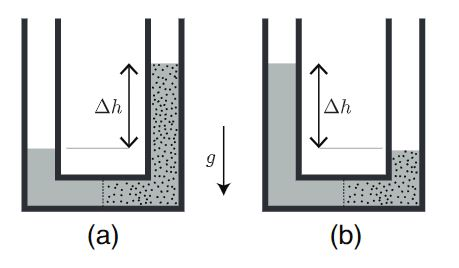
\includegraphics[height=7cm, width=11cm]{1.JPG}
        \end{center}

        \textcolor{hwColor}{
          I draw the plot with my hands so it is not really accurate and nice. I think it is a good fit based on the data based on 
          the values of $a$ and $b$. but it seems that the van de Waals is not giving very accurate result but does give a good approximation.
          \\
          \\
        }

    \end{enumerate}
    
    \item \textbf{1.18} Calculate the rms speed of a nitrogen molecule at room temperature.

        \textcolor{hwColor}{
          \\
          On page 13 we are given the formula for $v_{rms}$ so we have.
          $
            \\
            \\
            v_{rms}=\sqrt{\dfrac{3RT}{M}}=\sqrt{\dfrac{3 (8.31 ~ J/K) (300 ~ K)}{25 \times 10^{-3} ~ kg}}
            \\
            \\
            \\
            \therefore ~~~ \boxed{
              v_{rms} \approx 517 ~ m/s
            } ~~~~ \checkmark
            \\
          $
        }
    
    \item \textbf{1.22} If you poke a hole in a container full of gas, the gas will start leaking out. In this problem you 
    will make a rough estimate of the rate at which gas escapes through a hole. (This process is called \textbf{effusion}, at least when 
    the hole is sufficiently small.)

      \begin{enumerate}
        \item Consider a small portion (area=A) of the inside wall of a container full of gas. Show that the number of molecules colliding
        with this surface in a time interval $\Delta t$ is $P ~ A ~ \Delta t/(2m \overline{v_x})$, where $P$ is the pressure, $m$ is the 
        average molecular mass, and $\overline{v_x}$ is the average $x$ velocity of those molecules that collide with the wall.

          \textcolor{hwColor}{
            \\
            On page 11 we learned about $\bar{P}$, and also from equation 1.11 $(\Delta v_x)$. Assuming the collison between 
            molecules is an elastic one we have:
            \\
            \\
            $
              \begin{cases}
                P=N \bar{P} ~~~~ (\text{Totoal pressure}) 
                \\
                \\
                \bar{P}=-\dfrac{m ~ \Delta v_x}{A ~ \Delta t}
              \end{cases} \Longrightarrow 
              P=N \left[-\dfrac{m ~ \Delta v_x}{A ~ \Delta t}\right]
              \\
              \\
            $
            Using the value of $\Delta v_x=-2 \bar{v_x}$ we get:
            \\
            \\
            $
              P=-N \left[\dfrac{-m \times 2 \bar{v_x}}{A ~ \Delta t}\right]
              \\
              \\
              \\
              \therefore ~~~ \boxed{
                N=\dfrac{PA \Delta t}{2 m \bar{v_x}}
              } ~~~~ \checkmark ~~~~~~ \text{The number of molecules colliding}
              \\
              \\
            $ 
          }

        \item It is not easy to calculate $\overline{v_x}$, but a good enough approximation is $\overline{v_x}^{1/2}$, where the bar 
        now represents an average over all molecules in the gas. Show that $\overline{v_x}^{1/2}=\sqrt{kT/m}.$

          \textcolor{hwColor}{
            \\
            $
              \bar{P}=\sum\limits_{i=1}^{\infty} \dfrac{m v^2_{ix}}{V}
              \\
              \\
              \begin{cases}
                PV=N m \bar{v}^2_x
                \\
                \\
                PV=N K T
              \end{cases}
              \\
              \\
              \Longrightarrow N m \bar{v}^2_x=N K T 
              \\
              \\
              \\
              \therefore ~~~ \boxed{
                \sqrt{\bar{v}^2_x}=\sqrt{\dfrac{kT}{m}} \Leftrightarrow \bar{v}^2_x=\dfrac{kT}{m}
              } ~~~~ \checkmark
              \\
            $
          }
          
        \item If we now take away this small part of the wall of the container, the molecules that would have collided with it will 
        instead escape through the hole. Assuming that nothing enters through the hole, show that the number $N$ of molecules inside
        the container as a fucntion of time is governed by the differential equation
        $$
          \dfrac{dN}{dt}=-\dfrac{A}{2V} \sqrt{\dfrac{kT}{m}} N
        $$
        Solve this equation (assuming constant temperature) to obtain a formula of the form $N(t)=N(0) ~ e^{-t\tau}$, where $\tau$
        is the "characteristic time" for $N$ (and $P$) to drop by a factor of $e$.

          \textcolor{hwColor}{
            \\
            $
              -\Delta N=\dfrac{PA \Delta t}{2m} \sqrt{\dfrac{m}{kT}}
              =\dfrac{
                A \Delta t \times \bigg( \dfrac{NkT}{V} \bigg)
              }{
                2m
              } \sqrt{\dfrac{m}{kT}}
              \\
              \\
              \\
              \dfrac{\Delta N}{\Delta t}=-\dfrac{AN}{2V} \sqrt{\dfrac{m}{kT}}
              \\
              \\
              \text{When} \Delta t \Rightarrow 0, \text{then} ~  \dfrac{dN}{dt}=-\dfrac{AN}{2V} \sqrt{\dfrac{m}{kT}}=-\dfrac{1}{\tau} N
              \\
              \\
              \\
              \bigints\limits_{N(0)}^{N(t)} \dfrac{dN}{N}=-\bigints\limits_{0}^{t} \dfrac{dt}{\tau}
              \\
              \\
              \\
              \mathbf{ln} \left[\dfrac{N(t)}{N(0)} \right]=-\dfrac{t}{\tau} 
              \\
              \\
              \\
              \therefore ~~~ \boxed{
                N(t)=N(0) e^{-t/\tau}
              } ~~~~ \checkmark
              \\
            $
          }

        \pagebreak

        \item Calculate the characteristic time for a gas to escape from 1-liter container punctured by a $1-mm^2$ hole.
        
          \textcolor{hwColor}{
            \\
            $
              \dfrac{dN}{dt}=-\dfrac{1}{\tau} N
              \\
              \\
              \dfrac{A}{2V} \sqrt{\dfrac{kT}{m}}=\dfrac{1}{\tau}
              \\
              \\
              \\
              \sqrt{\dfrac{RT}{M}}=\sqrt{\dfrac{(8.3 ~ J.mol.K)(300 ~ K)}{29 \times 10^{-3}}} \approx 293 ~ m/s
              \\
              \\
              V=(1 lt) \left[1000 ~ m^3/1 lt\right]=0.001 ~ m^3
              \\
              \\
              \\
              A=(1 ~ mm^2) \left[1 ~ m/1000 ~ mm\right]=10^{-6} ~ m^2
              \\
              \\
              \tau=\dfrac{2V}{A} \sqrt{\dfrac{m}{kT}}=\dfrac{2(0.001 ~ m^3)}{(10^{-6})(293 ~ m/s)}
              \\
              \\
              \\
              \therefore ~~~ \boxed{
                \tau \approx 6.9 ~ s
              }
              \\
            $
          }

        \item Your bicycle tire has a slow leak, so that it goes flat within about an hour after being inflated. Roughly how big is the 
        hole? (Use any reasonable estimate for the volume of the tire.)

          \textcolor{hwColor}{
            \\
            $
              V=\pi (0.02 ~ m)^2 ~ (2m)=0.0025 ~ m^3, ~~~~ \tau=1 ~ hr= 3600 ~ s
              \\
              \\
              A=\dfrac{2V}{\tau \sqrt{RT/M}}=\dfrac{2(0.0025 ~ m^3)}{(3600 ~ s) (300 ~ m/s)}
              \\
              \\
              \\
              \therefore ~~~ \boxed{
                A=5 \times 10^{-9} ~ m^2
              } ~~~ \checkmark
              \\
            $
          }

        \item In Jules Verne's \emph{Round the Moon}, the escape travelers dispose of a dog's corpse by quickly opening a window,
        tossing it out, and closing the window. Do you think they can do this quickly enough to prevent a significant amount of air
        from escaping? Justify your answer with some rough estimates and calculation.

          \textcolor{hwColor}{
            \\
            $
              \tau=\dfrac{2V}{A\sqrt{RT/M}}=\dfrac{2(50 ~ m^3)}{0.2 ~ m^2 ~ \left(293 ~ m/s\right)}
              \\
              \\
              \\
              \therefore ~~~ \boxed{
                \tau=1.7 ~ s
              } ~~~~ \checkmark
            $
            \\
          }

      \end{enumerate}

  \end{enumerate}

\end{document}
